Laser modelocking -- Simon's self study problem set is a good starting point.

\begin{parts}
	\part Q-switching: the overpumping ratio $r = \dfrac{N_i^*}{N_\textnormal{th}^*}$, where $N_i^*$ is the initial population inversion before the pulse and $N_\textnormal{th}^*$ is the threshold population inversion, governs the Q pulse profile.
		
	$N_\textnormal{th}^*$ is dependent on the size of cavity and the population kinematics of the gain medium (i.e. the $\beta$ factor).
		
	Modelocking: multiple modes are synchronised in phase to produce an intense, short pulse.
	The bandwidth of the laser system, i.e. the number of modes in the cavity, governs the laser pulse length (strictly for inhomogeneous medium).
	
	Modelocking tends to produce short pulse length as it is easier to excite more modes than shortening the cavity length down to the \unit{\micro\metre} scale.
	
	\part Each mode have field component $E_p(t) = a(\omega_p) \mathrm{e}^{i(kz - \omega_p t + \phi_0)}$, setting the origin at the output coupler then gives the total field:
	\begin{align*}
		E(t) &= \sum_{p} a(\omega_p) \mathrm{e}^{-i(\omega_{ce} + p\Delta\omega)t} \mathrm{e}^{i\phi_0} \\
		&= \underbracket{\mathrm{e}^{-i(\omega_{ce} - \phi_0)}}_{\textnormal{carrier}} \underbracket{\sum_{p} a(\omega_p) \mathrm{e}^{-ip\Delta\omega t}}_{\textnormal{envelope}}
	\end{align*}
	
	The intensity is then:
	\begin{align*}
		I(t) &\propto \abs{E(t)}^2 \\
		&= \sum_{p} \sum_{q} a(\omega_p) a^*(\omega_q) \mathrm{e}^{-i(p-q)\Delta\omega t}
	\end{align*}
	
	Note that we have a maximum when $\Delta\omega t = 2\pi m$ where $m$ is an integer.
	Hence $t_m = \frac{2\pi}{\Delta\omega}m$.
	
	\begin{figure}[H]
		\centering
		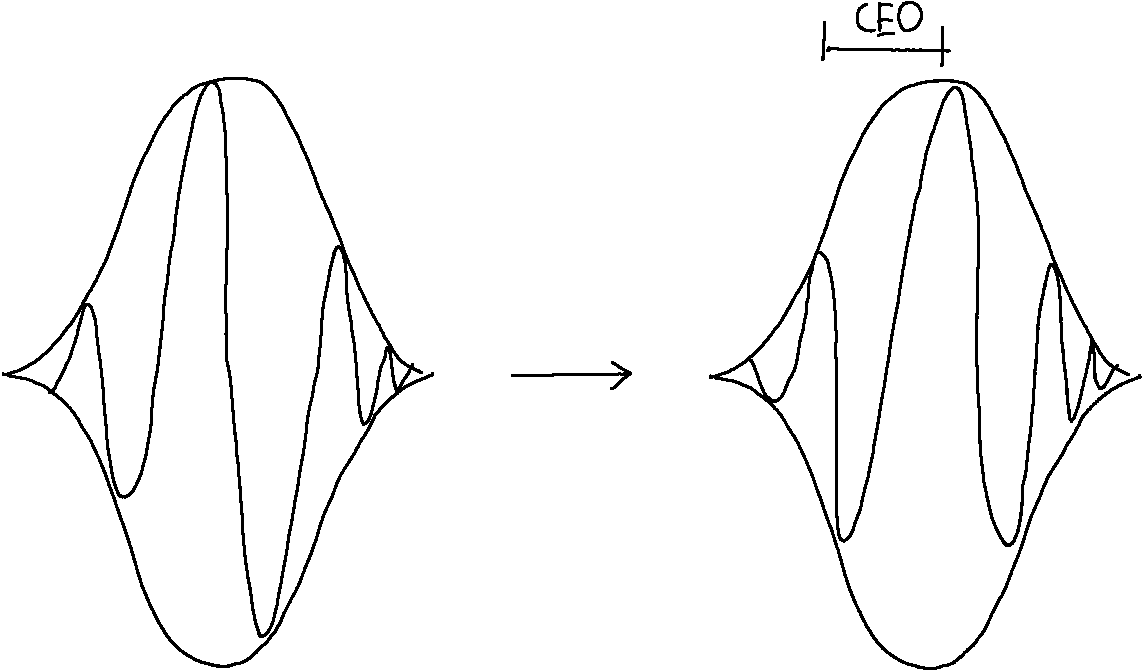
\includegraphics[width=.6\linewidth]{q1-ceo}
	\end{figure}
	
	CEO offset is the phase difference between the carrier wave and the envelope after 1 optical cycle, this is important when the envelope contains few carrier peaks (i.e. $\omega_{ce} \simeq \Delta\omega$).
	
	Substitute $t_m$ into $E(t)$ then gives:
	\begin{align*}
		E(t_m) &= \mathrm{e}^{-i(\frac{2\pi\omega_{ce}}{\Delta\omega} m - \phi_0)} \sum_{p} a(\omega_p) \mathrm{e}^{-ip \cdot 2\pi m} \\
		&= \mathrm{e}^{\phi_\textnormal{slip} \cdot m - \phi_0} \sum_{p} a(\omega_p) \mtext{where $\phi_\textnormal{slip} = \dfrac{2\pi\omega_{ce}}{\Delta\omega}$}
	\end{align*}
	
	\part From the given spectral component we have:
	\begin{equation*}
		a(\omega_p) = A \exp\sbracket{-\rbracket{\frac{p\Delta\omega + \omega_{ce} - \omega_0}{\Delta\omega_b}}^2}
	\end{equation*}
	
	The resulting E field is then:
	\begin{align*}
		E(t) &= \mathrm{e}^{-i(\omega_{ce} t - \phi_0)} \sum_{p} A \mathrm{e}^{-\rbracket{\frac{p\Delta\omega + \omega_{ce} - \omega_0}{\Delta\omega_b}}^2} \mathrm{e}^{-ip\Delta\omega t} \\
		&\simeq \mathrm{e}^{-i(\omega_{ce} t - \phi_0)} \frac{A}{\Delta\omega}
		\defint{-\infty}{\infty}{
			\mathrm{e}^{-\frac{\Omega^2}{\Delta\omega_b^2}} \mathrm{e}^{-i\Omega t} \mathrm{e}^{-i(\omega_{ce} + \omega_0)t}
		}{\Omega}
		\mtext{where \parbox[t]{10em}{$\Omega = p\Delta\omega + \omega_{ce} - \omega_0$ \\ $\inftsml{\Omega} = \inftsml{(p\Delta\omega)}$ \\ since $p$ is large and $a$ is bounded}} \\
		&= \mathrm{e}^{-i(\omega_{ce} t - \phi_0 - \omega_{ce} t + \omega_0 t)} \cdot \frac{A}{\Delta\omega} 
		\defint{-\infty}{\infty}{
			\mathrm{e}^{-\frac{1}{\Delta\omega_b^2} \Omega^2} \mathrm{e}^{-i\Omega t}
		}{\Omega} \\
		&= \frac{A}{\Delta\omega} \mathrm{e}^{-i(\omega_0 t - \phi_0)} \cdot \frac{\sqrt{\pi}}{1/\Delta\omega_b} \cdot \mathrm{e}^{-\rbracket{\frac{t}{2/\Delta\omega_b}}^2} \\
		&= \underbracket{\frac{A}{\Delta\omega} \sqrt{\pi} \Delta\omega_b \mathrm{e}^{-\rbracket{\Delta\omega_b t/2}^2}}_{F(t)} \underbracket{\mathrm{e}^{-i(\omega_0 t - \phi_0)}}_{\psi = \phi_0}
	\end{align*}
	
	Note that this form has no dependence on $\omega_{ce}$, it is only the parameter $\Delta\omega_b$ and $\omega_0$ that determines the temporal profile of the pulse.
	Also $E$ is inversely proportional to $\Delta\omega$.
	
	\part Frequency doubling $\omega_p \rightarrow 2\omega_p$ so we have:
	\begin{equation*}
		a(2\omega_p) = A \exp\sbracket{-\rbracket{\frac{2p\Delta\omega + 2\omega_{ce} - \omega_0}{\Delta\omega_b}}}
	\end{equation*}
	
	\begin{figure}[H]
		\centering
		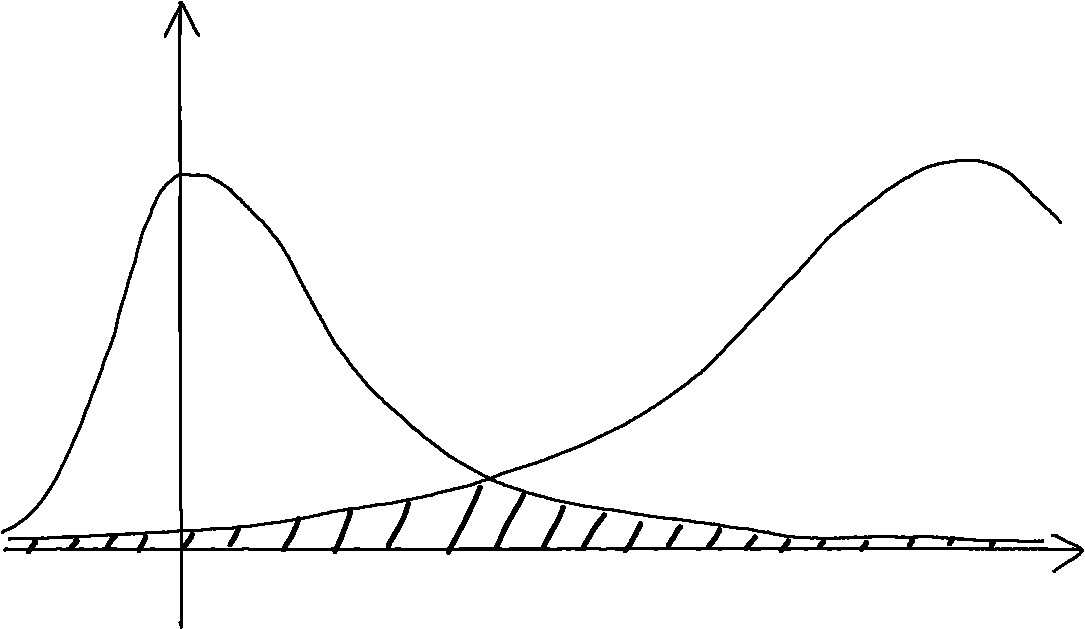
\includegraphics[width=.6\linewidth]{q1-freq-doubling}
	\end{figure}
	
	Noting the Gaussian form and letting $\Delta\omega_b$ goes large shows that there will be an overlap between the 2 spectrum, the minimum frequency difference is simply between like $p$'s:
	\begin{equation*}
		2\omega_{ce} - \omega_0 - \omega_{ce} + \omega_0 = \omega_{ce}
	\end{equation*}
	
	To achieve $\phi_\textnormal{slip} = 0$, we may frequency double the output, measure the beating frequency between it and the original output, and adjust the cavity length such that there is no longer any beating, suggesting that $\omega_{ce} = 0 \Rightarrow \phi_\textnormal{slip} = 0$.
\end{parts}